% Created by tikzDevice version 0.10.1 on 2017-10-23 14:01:34
% !TEX encoding = UTF-8 Unicode
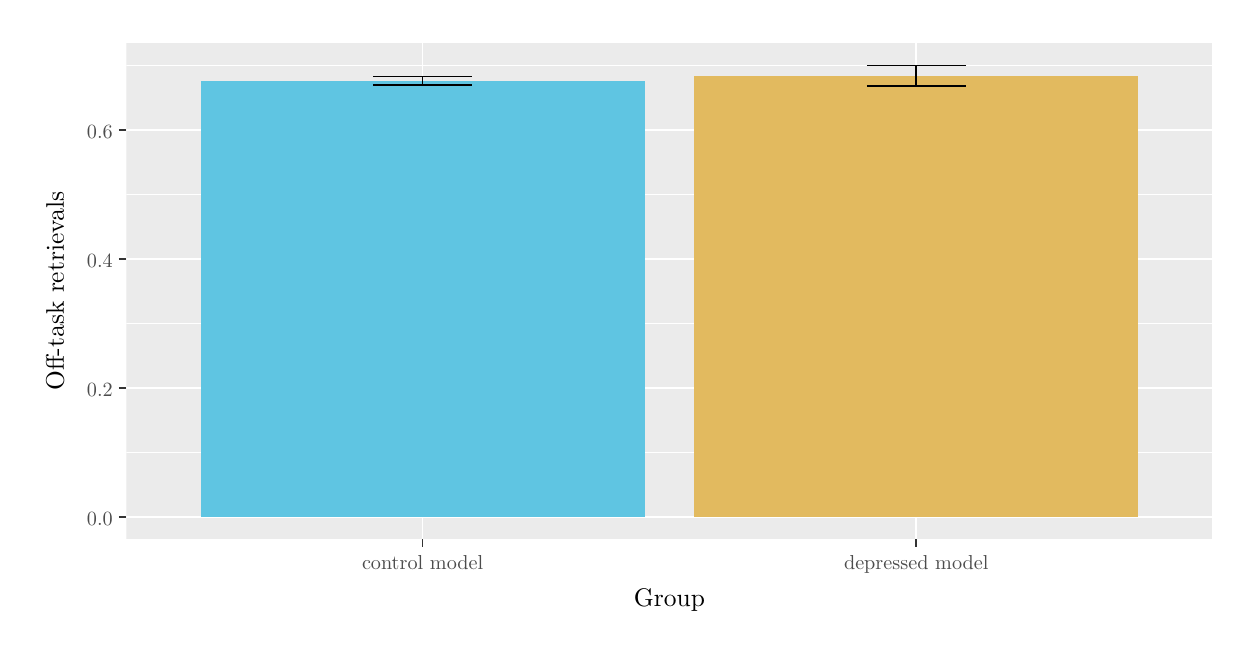
\begin{tikzpicture}[x=1pt,y=1pt]
\definecolor{fillColor}{RGB}{255,255,255}
\path[use as bounding box,fill=fillColor,fill opacity=0.00] (0,0) rectangle (433.62,216.81);
\begin{scope}
\path[clip] (  0.00,  0.00) rectangle (433.62,216.81);
\definecolor{drawColor}{RGB}{255,255,255}
\definecolor{fillColor}{RGB}{255,255,255}

\path[draw=drawColor,line width= 0.6pt,line join=round,line cap=round,fill=fillColor] (  0.00,  0.00) rectangle (433.62,216.81);
\end{scope}
\begin{scope}
\path[clip] ( 35.70, 31.92) rectangle (428.12,211.31);
\definecolor{fillColor}{gray}{0.92}

\path[fill=fillColor] ( 35.70, 31.92) rectangle (428.12,211.31);
\definecolor{drawColor}{RGB}{255,255,255}

\path[draw=drawColor,line width= 0.3pt,line join=round] ( 35.70, 63.37) --
	(428.12, 63.37);

\path[draw=drawColor,line width= 0.3pt,line join=round] ( 35.70,109.96) --
	(428.12,109.96);

\path[draw=drawColor,line width= 0.3pt,line join=round] ( 35.70,156.55) --
	(428.12,156.55);

\path[draw=drawColor,line width= 0.3pt,line join=round] ( 35.70,203.15) --
	(428.12,203.15);

\path[draw=drawColor,line width= 0.6pt,line join=round] ( 35.70, 40.07) --
	(428.12, 40.07);

\path[draw=drawColor,line width= 0.6pt,line join=round] ( 35.70, 86.67) --
	(428.12, 86.67);

\path[draw=drawColor,line width= 0.6pt,line join=round] ( 35.70,133.26) --
	(428.12,133.26);

\path[draw=drawColor,line width= 0.6pt,line join=round] ( 35.70,179.85) --
	(428.12,179.85);

\path[draw=drawColor,line width= 0.6pt,line join=round] (142.72, 31.92) --
	(142.72,211.31);

\path[draw=drawColor,line width= 0.6pt,line join=round] (321.10, 31.92) --
	(321.10,211.31);
\definecolor{fillColor}{RGB}{95,197,226}

\path[fill=fillColor] ( 62.46, 40.07) rectangle (222.99,197.61);
\definecolor{fillColor}{RGB}{226,186,95}

\path[fill=fillColor] (240.83, 40.07) rectangle (401.36,199.40);
\definecolor{drawColor}{RGB}{0,0,0}

\path[draw=drawColor,line width= 0.6pt,line join=round] (124.89,199.18) --
	(160.56,199.18);

\path[draw=drawColor,line width= 0.6pt,line join=round] (142.72,199.18) --
	(142.72,196.04);

\path[draw=drawColor,line width= 0.6pt,line join=round] (124.89,196.04) --
	(160.56,196.04);

\path[draw=drawColor,line width= 0.6pt,line join=round] (303.26,203.16) --
	(338.93,203.16);

\path[draw=drawColor,line width= 0.6pt,line join=round] (321.10,203.16) --
	(321.10,195.65);

\path[draw=drawColor,line width= 0.6pt,line join=round] (303.26,195.65) --
	(338.93,195.65);
\end{scope}
\begin{scope}
\path[clip] (  0.00,  0.00) rectangle (433.62,216.81);
\definecolor{drawColor}{gray}{0.30}

\node[text=drawColor,anchor=base east,inner sep=0pt, outer sep=0pt, scale=  0.73] at ( 30.75, 37.04) {0.0};

\node[text=drawColor,anchor=base east,inner sep=0pt, outer sep=0pt, scale=  0.73] at ( 30.75, 83.64) {0.2};

\node[text=drawColor,anchor=base east,inner sep=0pt, outer sep=0pt, scale=  0.73] at ( 30.75,130.23) {0.4};

\node[text=drawColor,anchor=base east,inner sep=0pt, outer sep=0pt, scale=  0.73] at ( 30.75,176.82) {0.6};
\end{scope}
\begin{scope}
\path[clip] (  0.00,  0.00) rectangle (433.62,216.81);
\definecolor{drawColor}{gray}{0.20}

\path[draw=drawColor,line width= 0.6pt,line join=round] ( 32.95, 40.07) --
	( 35.70, 40.07);

\path[draw=drawColor,line width= 0.6pt,line join=round] ( 32.95, 86.67) --
	( 35.70, 86.67);

\path[draw=drawColor,line width= 0.6pt,line join=round] ( 32.95,133.26) --
	( 35.70,133.26);

\path[draw=drawColor,line width= 0.6pt,line join=round] ( 32.95,179.85) --
	( 35.70,179.85);
\end{scope}
\begin{scope}
\path[clip] (  0.00,  0.00) rectangle (433.62,216.81);
\definecolor{drawColor}{gray}{0.20}

\path[draw=drawColor,line width= 0.6pt,line join=round] (142.72, 29.17) --
	(142.72, 31.92);

\path[draw=drawColor,line width= 0.6pt,line join=round] (321.10, 29.17) --
	(321.10, 31.92);
\end{scope}
\begin{scope}
\path[clip] (  0.00,  0.00) rectangle (433.62,216.81);
\definecolor{drawColor}{gray}{0.30}

\node[text=drawColor,anchor=base,inner sep=0pt, outer sep=0pt, scale=  0.73] at (142.72, 20.91) {control model};

\node[text=drawColor,anchor=base,inner sep=0pt, outer sep=0pt, scale=  0.73] at (321.10, 20.91) {depressed model};
\end{scope}
\begin{scope}
\path[clip] (  0.00,  0.00) rectangle (433.62,216.81);
\definecolor{drawColor}{RGB}{0,0,0}

\node[text=drawColor,anchor=base,inner sep=0pt, outer sep=0pt, scale=  0.92] at (231.91,  7.83) {Group};
\end{scope}
\begin{scope}
\path[clip] (  0.00,  0.00) rectangle (433.62,216.81);
\definecolor{drawColor}{RGB}{0,0,0}

\node[text=drawColor,rotate= 90.00,anchor=base,inner sep=0pt, outer sep=0pt, scale=  0.92] at ( 13.08,121.61) {Off-task retrievals};
\end{scope}
\end{tikzpicture}
